\chapter{Software OpenSource y Libre}
		\subsection{Deferencias} 
Una interpretación de lo que se entiende por el término \textit{open source}, cuando se utiliza en el contexto de la descripción de un programa de software o diseño de hardware, es que el código fuente del diseño se encuentra disponible a la vista de alguna forma. A pesar de que es una amplia y potencialmente término ambiguo , un común acuerdo sobre la definición está en un documento llamado la Open Source Definition (OSD ), publicado por la Open Source Initiative (OSI).
Una interpretación sencilla de lo que se entiende por el término open source , cuando se utiliza en el contexto de la descripción de un programa de software o diseño de hardware , es que el diseño Fuentes de alguna manera están disponibles a la vista. A pesar de que es un amplio y potencial término ambiguo, un común acuerdo sobre la definición está en un documento llamado  Open Source Definition (OSD ), publicado por la Open Source Initiative (OSI).

La definición no es una licencia de software libre en sí, si no algo para medir condiciones frente a la distribución para determinar si cumplen y, si lo hacen, entonces se puede decir que es \textit{open source}\cite{Etiqueta06}.La definición no es una licencia de software libre en sí, si no algo para medir condiciones frente a la distribución para determinar si cumplen y, si lo hacen, entonces se puede decir que es \textit{open source}. Cuando el software \textit{libre} o \textit{free} se utiliza para describir el software de código abierto, se refiere a los derechos y no al costo del usuario. La Fundación para el Software Libre (FSF) ofrece una definición para mostrar claramente qué se tiene que cumplir sobre el software para que pueda ser considerado libre \cite{Etiqueta07}. El termino Free Software Foundation (FOSS) es usado para referirse al software que se adhiere al OSD y FSF. El software libre y de código abierto es una sociedad inclusiva término que abarca tanto el software libre y software de código abierto que a pesar de describir modelos de desarrollo similares, tienen diferentes culturas y filosofías.

El software \textit{libre} se refiere a la libertad de los usuarios para ejecutar, copiar, distribuir, estudiar, cambiar y mejorar el software. El vocablo \textit{free} en ingles significa :gratis y/o libre. Por ello el término ha ocasionado confusiones dándose a entender, equivocadamente, que el software libre es gratuito o regalado. Pero no es una cuestión de presencia o ausencia de costo, puesto que el software libre no significa que no pueda ser comercial.

Stallman fundó la Free Software Foundation (FSF ) en 1985 para promover la libertad del usuario y para defender los derechos de todo el software libre( 28 ). La FSF patrocina el proyecto GNU. El software libre permite al usuario el ejercicio de cuatro libertades básicas:

\begin {itemize}
\item
 \textit{Libertad 0} Además el software \textit{libre} permite estudiar cómo funcionan y adaptarlo a las necesidades de quien lo use. Tener acceso a su código fuente posibilita, entre otras cosas, descubrir qué posibilidades tiene, etc. El adaptar el programa a las necesidades del usuario se puede suprimir partes que no le interesen, agregar otras partes que considere importantesm copiar una parte que realiza una tarea y/o adicinarla a otro programa, etc.

\item
\textit{Libertad 1} El software, sus copias y las modificaciones se pueden distribuir libremente, lo que significa poseer la libertad de redistribuir el programa, gratis o con algún costo, ya sea por mail, FTP, o en CD, redistibuyéndolo a una persona o a varias, a una persona que vive en otro país, etc.

\item 
\textit{Libertad 2} Es posible mejorarlo y hacer pública esas mejoras. La libretad de hacer un programa mejor, implica que se puede hacer menores los requerimientos de hardware para funcionar, que tenga mayores prestaciones, que sus requerimientos no sean tan altos, que tenga menos errores, etc. El poder liberar las mejoras al público quiere decir que si se realiza una mejora que permita un requerimiento menor de hardware, o que haga que ocupe menos espacio, se puede redistribuir ese programa mejorando o simplenete propoenr la mejora en lugar público (un foro de noticias, una lista de correo, un sitio web, un FTP, un canal de chat).

\item 
\textit{Libertad 3} El usuario al poseer el código fuente tiene poder de decisón, ya que podrá elegir quién puede modifica los programas que ha adquirido para mejorarlos (o bien mejorarlos el mismo). Es decir esto permite que no exista un monopolio, porque en el caso de que un software sea discontinuado el usuario podrá nuevamente (al poseer el código) elegir a un desarrollador para continuar utilizando el software que fue discontinuado. Además el usuario no estará completamente a merced de tener que renovar su hardware y software constantemente según ocurre a menudo con las políticas de las empresas que producen software privativo y también será libre de vender o redistribuir software libre.
 
 \end {itemize}
 
Mediante la licencias un autor permite el uso de su creación a otras personas, de la manera que el cree aceptable. En ese sentido la licencia es el intrumento que regula las maneras en que el usuario puede utilizar el software.

También una licencia de software es un contrato que determina en qué condiciones el usuario puede utilizar el programa informático y qué obligaciones asquiere para su uso. Cuando se instala un programa informático, o a veces, incluso, por el simple hecho de abrir el sobre que lo contiene, se esta aceptando las condiciones de su licencia de software.

Cuando IBM comenzó la venta de computadoras a gran escala en la década de 1960, el software venia incluido como código fuente. Una década más tarde, sin embargo, comenzaron a "desagregar"  el software, y se convirtió en habitual para los fabricantes de computadoras, no solo limito  el uso del mismo código fuente a los competidores, sino que también elimino la capacidad de modificar el código libremente y compartirlo%\cita{}(26).  

La licencia División de Software de Berkeley (BSD) y la Pública General del proyecto GNU (GNU GPL) son dos de las primeras licencias de código abierto. Ambos proporcionan la libertad de usar software de código fuente abierto para cualquier propósito y permitir la modificación y la distribución de su código fuente sin tener que pagar regalías. Las diferencias entre los dos pone de relieve una diferencia ideológica entre los defensores del código abierto .

Un punto significativo de diferencia entre las licencias BSD y GPL es que este último le permite
\textit{modificar su copia o copias del Programa o cualquier parte de el, y copie
y distribuir tales modificaciones ... supuesto que además ... hace que la
totalidad de cualquier trabajo que distribuya o publique y que en todo o en
parte contenga el Programa o cualquier parte del mismo, ya sea con o sin
modificaciones, para ser autorizadas sin cargo alguno para terceras partes bajo el
términos de esta Licencia Pública General.(GPLv1) ( 29 ). } %\cita{}

La GNU GPL se conoce como una licencia \textit{viral}, en que cualquier diseño haciendo uso de código ya licenciado bajo la GNU GPL debe ser entonces licenciado bajo la
GNU GPL o cualquier licencia juzgados como igualmente sin restricciones por la FSF. En pocas palabras, una condición de uso del código licenciado bajo GPL es que su diseño se debe tener licencia bajo la GPL o una licencia compatible. Las licencias que se consideran compatibles con la GPL por la FSF son generalmente similares en las libertades que garantiza el software libres. La licencia se transmite al código que hacen uso de ella. El GNU GPLv3 exige que cuando un proyecto adopta esta licencia el código fuente debe estar disponible y que las patentes o derechos digitales (DRM) no inhiben a otros del uso del diseño. 

La licencia BSD modificada es básicamente la misma que la original sin la clausula de publicidad. De acuerdo con dicha cláusula, todo el material de publicidad en el cual se menciona características o la utilización de este software tenia que mostrar el siguiente asentimiento:"este producto incluye software desarrollado por la Universidad de California, Berkeley y sus contribuyentes ".

Esta cláusula de publicidad no permitía que fuera compatible con la lincencia GPL pero a partir de su versión 2.0 fue eliminada y la licencia pasó a ser compatible con la GPL.

La GNU GPL es en cierto modo, más restrictiva que la licencia BSD sobre las libertad de hacer lo que uno quiere con el código fuente. En la GNU se estipula que el código modificado debe estar disponible, y cualquier diseño utilizado con código GPL tiene también que venir bajo la GNU GPL. Sin embargo, esto no es diferente a cualquier licencia comercial, donde el código fuente escrito por un empleado de una empresa,o todo el código que se modifican o crean esta bajo la licencia exclusiva de la empresa. En el caso de la licencia de GNU, sin embargo, los usuarios están obligados a mantener su diseño abierto y libre como la GPL de GNU hace, de la misma manera el empleado de la empresa está obligado a mantener su código propietario en secreto para cualquiera que no sea de la  empresa.

Otro punto de controversia es el uso combinado de los diseños en los que cada uno es bajo
una licencia diferente, ha dado lugar al concepto de \textit{compatibilidad de la licencia}. El significado de uso aquí es ambiguo y depende del contexto

		\subsection{OpenSource}

		\subsection{¿Quien tiene el Hardware?}

		\subsection{OpenRISC}



%\cite{Etiqueta02},
%\textit{FPGAs}) .
%\begin {itemize}
%\item  Bloques lógicos configurables y \textit{Lookup Tables}.
% \end {itemize}

\begin{figure}[h!]
 \begin{center}
  % 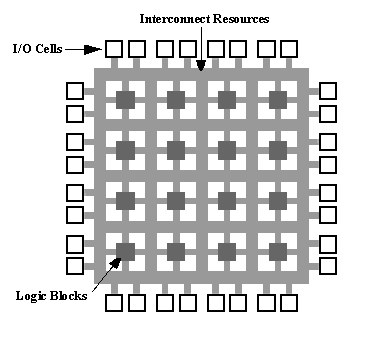
\includegraphics[width=0.5\textwidth,keepaspectratio=true]{./images/fpga1a}
  \caption{Componentes de una FPGA}
  \label{fig:esquema}
 \end{center}
\end{figure}


%Conclusión!!Trabajar con un sistema final bajo licencias de hardware siguiendo el modelo de la Licencia LGPL para el software. Estamos comprometidos con el ideal de libre disposición, de libre uso y hardware de código abierto reutilizable.

